\documentclass[12pt,a4paper]{report}
\parindent =0cm
\usepackage{amsmath}
\usepackage{amssymb,amsfonts, 
latexsym,cancel}
\usepackage{array}
\usepackage{bm}
\usepackage{float}
\usepackage{fancyhdr}
\usepackage{graphicx}
\usepackage{epstopdf}
\usepackage[colorlinks = true,
			linkcolor = black,
			citecolor = black,
			urlcolor = blue]{hyperref}
\usepackage{longtable}
\setcounter{MaxMatrixCols}{40}
\usepackage{multicol}
\usepackage{subfigure}
\usepackage{titling}
\usepackage{titlesec}
\usepackage{setspace}
\newcolumntype{E}{>{$}c<{$}}

\usepackage{anyfontsize}
\usepackage[utf8]{inputenc}
\usepackage{amsmath}
\usepackage{amsfonts}
\usepackage{amssymb}
\usepackage{makeidx}
\usepackage{graphicx}
%\usepackage{fourier}

\setcounter{MaxMatrixCols}{100}
\usepackage[left=2cm,right=2cm,top=2cm,bottom=2cm]{geometry}
\author{Guadalupe Monroy}
\begin{document}
\thispagestyle{empty} %% PARA QUITAR FORMATO DE PIES Y 
%\fbox{
\begin{minipage}[c][0.15\textheight][c]{0.17\textwidth}
    \begin{center}
        
\includegraphics[height=2.2cm, keepaspectratio=true]{imagenes/logocp} %% LOGO IZQUIERDO
    \end{center}
\end{minipage}
%}
%\fbox{
\begin{minipage}[c][0.15\textheight][t]{0.9\textwidth}
    \begin{center}
        {\scshape \Huge COLEGIO DE POSTGRADUADOS} %% NOMBRE DE LA UNIVERSIDAD
        \vspace{.5cm}   %% DEFINE EL ESPACIO ENTRE EL NOMBRE DE LA UNIVERSIDAD Y LA LÍNEA DOBLE
        \hrule height2.5pt  %% DEFINE EL ANCHO DE LA PRIMER LÍNEA
        \vspace{.1cm}    %% DEFINE EL ESPACIO ENTRE LAS DOS LINEAS
        \hrule height1pt  %% DEFINE EL ANCHO DE LA SEGUNDA LINEA (NORMALMENTE ES MAS DELGADA)
        \vspace{.4cm}   %% DEFINE EL ESPACIO ENTRE LA DOBLE LINEA Y EL NOMBRE DE LA DIVISIÓN
        {\scshape \LARGE  CAMPUS MONTECILLO}  %% NOMBRE DE LA DIVISIÓN
    \end{center}
\end{minipage}
%}

%\fbox{
\begin{minipage}[l][0.78\textheight][t]{0.1\textwidth}
    \begin{center}
    \hskip0pt
    \vrule width2.5pt height17cm    %% height definde la altura de la linea gruesa
        \hskip1mm
        \vrule width1pt height17cm  %% height define la altura de la linea delgada
        \end{center}
\end{minipage}
%}
%\fbox{
\begin{minipage}[c][0.78\textheight][t]{0.8\textwidth}
      \begin{center}
      \vspace{2cm}
        {\Large \scshape {PSEI-ESTADÍSTICA Y CIENCIA DE DATOS}}

        \vspace{2cm}

        \makebox[5cm][c]{\LARGE Examen. MODELOS LINEALES}  \\[16pt]
        PROFESOR DR. HUMBERTO VAQUERA HUERTA             \\[15pt]
        {\Large \textbf{{}}}\\[25pt]
        Al:\\[12pt]
        \textbf{ \Large {Guadalupe Monroy Hernández}}

        \vspace{2cm}
        
        \vspace{2.5cm}

        { Texcoco, Edo. México} \hskip2.5cm {}
      \end{center}
\end{minipage}
%}

%--------EJERCICIO 1------------
\paragraph{Problema 1} (Distribucion de formas cuadraticas)

\begin{enumerate}
			
		\item Suponga que $X = \begin{pmatrix} X_1 \\ X_2 \\ X_3 \end{pmatrix}$ donde $X \sim N(\mu, \Sigma)$ donde $\mu = \begin{pmatrix} 3 \\ -2 \\ 1 \end{pmatrix}$, $\Sigma = \sigma^2 I = \begin{pmatrix} \sigma^2_{1} & 0 & 0 \\ 0 & \sigma^2_{2} & 0 \\ 0 & 0 & \sigma^2_{3} \end{pmatrix}$ y
			$A = \frac{1}{3} \begin{pmatrix} 2 & -1 & -1 \\ -1 & 2 & -1 \\ -1 & -1 & 2 \end{pmatrix}$, $B = \begin{pmatrix} 1 & 1 & 1 \\ 1 & 0 & -1 \end{pmatrix}$.

a. ¿Cuál es la distribución de $X^TAX/\sigma^2$?
			
Para $X\sim N_{n}(\mu, I)$, entonces:
		\begin{eqnarray*}
			X^{t}AX/\sigma^{2}&\sim& \it{X^{2}}(r,\mu'A\mu/2\sigma^{2})
		\end{eqnarray*}

Lo anterior si $A$ es simétrico e idempotente. Dado que $\Sigma$ es una matriz diagonal. \\
Pruea de idempotencia:\\ 
		
		\begin{eqnarray*}
		A^{2}&=&A  A=A\\
		&=&\frac{1}{3}  \begin{bmatrix}
				2 & -1 & -1\\
				-1 & 2 & -1\\
				-1 & -1 & 2\\
			\end{bmatrix}	
			\frac{1}{3}  \begin{bmatrix}
				2 & -1 & -1\\
				-1 & 2 & -1\\
				-1 & -1 & 2\\
			\end{bmatrix}\\			
			A^{2}&=&\begin{bmatrix}
				2/3 & -1/3 & -1/3\\
				-1/3 & 2/3 & -1/3\\
				-1/3 & -1/3 & 2/3
			\end{bmatrix}	
			\begin{bmatrix}
				2/3 & -1/3 & -1/3\\
				-1/3 & 2/3 & -1/3\\
				-1/3 & -1/3 & 2/3
			\end{bmatrix}\\
			&=&\begin{bmatrix}
				2/3 & -1/3 & -1/3\\
				-1/3 & 2/3 & -1/3\\
				-1/3 & -1/3 & 2/3
			\end{bmatrix}=A	\\						&&\therefore 	\textbf{A es idempotente, simétrica y con r=2}
		\end{eqnarray*}


		\begin{eqnarray*}
			X^{t}AX/\sigma^{2}&\sim& \it{X^{2}}(r,\mu'A\mu/2\sigma^{2})
		\end{eqnarray*}
		Se obtienen los parametros $\mu'A\mu/2\sigma^{2}$\\		
		\begin{eqnarray*}
			\mu'A\mu &=&\begin{bmatrix}
				3 & -2 & 1
			\end{bmatrix}	 
			\begin{bmatrix}
				2/3 & -1/3 & -1/3\\
				-1/3 & 2/3 & -1/3\\
				-1/3 & -1/3 & 2/3
			\end{bmatrix}
			\begin{bmatrix}
				3 \\
				-2  \\
				1 
			\end{bmatrix}=\dfrac{38}{3}			
		\end{eqnarray*}
		Por lo que $\mu'A\mu/2\sigma^{2}$:
		\begin{eqnarray*}
			\mu'A\mu/2\sigma^{2}&=&\dfrac{38}{\dfrac{3}{2\sigma^{2}}}=\dfrac{19}{3\sigma^{2}}
		\end{eqnarray*}
		La distribución es:
		\begin{eqnarray*}
		X^{t}AX/\sigma^{2}&\sim& \it{X^{2}}(2,\dfrac{19}{3\sigma^{2}})
		\end{eqnarray*}
		\\

b. ¿Son $X^TAX$ y $BX$ independientes?\\

Haciendo uno de la propiedad: Si B es una matriz de constantes k x p, A es una matriz simétrica de constantes p x p, y $X\sim N_{p}(\mu, \Sigma)$, entonces $BX$ y $X^{t}AX$ son independientes si y solo si $B\Sigma A=0$.
		
		\begin{eqnarray*}
			B\Sigma A&=&\begin{bmatrix}
				1 & 1 & 1\\
				1 & 0 & -1
			\end{bmatrix}	
			\begin{bmatrix}
				\sigma^{2}_{1} & 0 & 0\\
				0 & \sigma^{2}_{2} & 0\\
				0 & 0 & \sigma^{2}_{3}
			\end{bmatrix}
\dfrac{1}{3}
			\begin{bmatrix}
			2 & -1 & -1\\
			-1 & 2 & -1\\
			-1 & -1 & 2\\
		\end{bmatrix}\\
		&=& \dfrac{1}{3}
		\begin{bmatrix}
			\sigma^{2}_{1} & \sigma^{2}_{2} & \sigma^{2}_{3}\\
			\sigma^{2}_{1} & 0 & -\sigma^{2}_{3}
		\end{bmatrix}
		\begin{bmatrix}
			2 & -1 & -1\\
			-1 & 2 & -1\\
			-1 & -1 & 2\\
		\end{bmatrix}\\
		&=&\dfrac{1}{3} \begin{bmatrix}
			2\sigma^{2}_{1}- \sigma^{2}_{2} - \sigma^{2}_{3} & -\sigma^{2}_{1}+2\sigma^{2}_{2} - \sigma^{2}_{3}  & -\sigma^{2}_{1} - \sigma^{2}_{2} + 2\sigma^{2}_{3}\\
			2\sigma^{2}_{1} +\sigma^{2}_{3}  & -\sigma^{2}_{1} +\sigma^{2}_{3}  & -\sigma^{2}_{1} -2\sigma^{2}_{3} 
		\end{bmatrix} \neq 0\\
		&&\therefore\textbf{Por lo que no son independientes}
	\end{eqnarray*} 

c. ¿Son $X^TAX$ y $X_1 + X_2 + X_3$ independientes?\\

	Para definir si $X^TAX$ y $X_1 + X_2 + X_3$ son independientes \\
	

d. Suponga $C = \frac{1}{3} \begin{pmatrix} 1 & 1 & 1 \\ 1 & 1 & 1 \\ 1 & 1 & 1 \end{pmatrix}$. ¿Cuál es la distribución de $X^TCX/\sigma^2$?\\


	 \begin{eqnarray*} C&=& \dfrac{1}{3} \cdot
	 	\begin{pmatrix} 1 & 1 & 1 \\
	 		 			1 & 1 & 1 \\ 1 & 1 & 1 
		\end{pmatrix}
	 \end{eqnarray*}
Si $X\sim N_{n}(\mu, I)$, entonces
	 \begin{eqnarray*}
	 	X^{t}AX/\sigma^{2}&\sim& \it{X^{2}}(r,\mu'A\mu/2\sigma^{2})
	 \end{eqnarray*}
Prueba de idempotencia	 
	 \begin{eqnarray*}
	 	C^{2}&=& C\\
	 	&=&\frac{1}{3}  \begin{bmatrix}
	 		1 & 1 & 1\\
	 		1 & 1 & 1\\
	 		1 & 1 & 1\\
	 	\end{bmatrix}	
	 	\frac{1}{3}  \begin{bmatrix}
	 		1 & 1 & 1\\
	 		1 & 1 & 1\\
	 		1 & 1 & 1\\
	 	\end{bmatrix}
	 	=	\frac{1}{9}	\begin{bmatrix}
	 		3 & 3 & 3\\
	 		3 & 3 & 3\\
	 		3 & 3 & 3\\
	 	\end{bmatrix} \\
	 	&=&	\frac{1}{3} \cdot \begin{bmatrix}
	 		1 & 1 & 1\\
	 		1 & 1 & 1\\
	 		1 & 1 & 1\\
	 	\end{bmatrix} =C \quad \therefore \quad \textbf{es idempotente y de r=1}
	 \end{eqnarray*}
Se obtiene la distribución $X^{t}CX/\sigma^{2}\sim \it{X^{2}}(r,\mu'C\mu/2\sigma^{2})$
	\begin{eqnarray*}
		\mu'C\mu/2\sigma^{2} &=&\dfrac{1}{2\sigma^{2}} \cdot \begin{bmatrix}
			3 & -2 & 1
		\end{bmatrix}	
		\cdot 
		\begin{bmatrix}
			1/3 & 1/3 & 1/3\\
			1/3 & 1/3 & 1/3\\
			1/3 & 1/3 & 1/3
		\end{bmatrix}
		\cdot
		\begin{bmatrix}
			3 \\
			-2  \\
			1 
		\end{bmatrix}\\
		&=& \dfrac{1}{2\sigma^{2}} \cdot \begin{bmatrix}
			2/3 & 2/3 & 2/3
		\end{bmatrix}	\cdot
		\begin{bmatrix}
		3 \\
		-2  \\
		1 
		\end{bmatrix} = \dfrac{1}{2\sigma^{2}} \cdot \dfrac{4}{3} = \dfrac{2}{3\sigma^{2}}
	\end{eqnarray*}
La distribución es:
	\begin{eqnarray*}
		\mu'C\mu/2\sigma^{2} \sim X^{2} \left(1,\dfrac{2}{3\sigma^{2}}\right)
	\end{eqnarray*} 
	
e. ¿Son las formas cuadráticas $X^TAX$ y $X^TCX$ independientes?\\

$\mu'A\mu/2\sigma^{2}$ y $\mu'C\mu/2\sigma^{2}$ son independientes si $B\Sigma A=0$
	
	\begin{eqnarray*}
	B\Sigma A&=&\begin{bmatrix}
	1/3 & 1/3 & 1/3\\
	1/3 & 1/3 & 1/3\\
	1/3 & 1/3 & 1/3
\end{bmatrix}	
\cdot 
\begin{bmatrix}
	\sigma^{2}_{1} & 0 & 0\\
	0 & \sigma^{2}_{2} & 0\\
	0 & 0 & \sigma^{2}_{3}
\end{bmatrix}
\cdot 
\begin{bmatrix}
	2/3 & -1/3 & -1/3\\
	-1/3 & 2/3 & -1/3\\
	-1/3 & -1/3 & 2/3\\
\end{bmatrix}\\
&=&\begin{bmatrix}
	1/3 \sigma_{1}^{2} & 1/3 \sigma_{2}^{2} & 1/3 \sigma_{3}^{2}\\
	1/3 \sigma_{1}^{2} & 1/3 \sigma_{2}^{2} & 1/3 \sigma_{3}^{2} \\
	1/3 \sigma_{1}^{2} & 1/3 \sigma_{2}^{2} & 1/3 \sigma_{3}^{2}
\end{bmatrix}	
\cdot 
\begin{bmatrix}
	2/3 & -1/3 & -1/3\\
	-1/3 & 2/3 & -1/3\\
	-1/3 & -1/3 & 2/3\\
\end{bmatrix}\\
&=& \begin{bmatrix}
	2/9 \sigma_{1}^{2} - 1/9 \sigma_{2}^{2} - 1/9 \sigma_{3}^{2}  & -1/9 \sigma_{1}^{2} + 2/9 \sigma_{2}^{2} - 1/9 \sigma_{3}^{2} & -1/9 \sigma_{1}^{2} - 1/9 \sigma_{2}^{2} + 2/9 \sigma_{3}^{2}\\
	2/9 \sigma_{1}^{2} - 1/9 \sigma_{2}^{2} - 1/9 \sigma_{3}^{2}  & -1/9 \sigma_{1}^{2} + 2/9 \sigma_{2}^{2} - 1/9 \sigma_{3}^{2} & -1/9 \sigma_{1}^{2} - 1/9 \sigma_{2}^{2} + 2/9 \sigma_{3}^{2} \\
	2/9 \sigma_{1}^{2} - 1/9 \sigma_{2}^{2} - 1/9 \sigma_{3}^{2}  & -1/9 \sigma_{1}^{2} + 2/9 \sigma_{2}^{2} - 1/9 \sigma_{3}^{2} & -1/9 \sigma_{1}^{2} - 1/9 \sigma_{2}^{2} + 2/9 \sigma_{3}^{2}
\end{bmatrix}\neq 0
	\end{eqnarray*}
\end{enumerate}


%--------EJERCICIO 3_1------------
\paragraph{Problema 2}  (Teorema de Cochran).\\

 Sean 
 \begin{align*}
 B_1 = \dfrac{1}{6}
 \begin{bmatrix}
 2  & 2  & -1 & -1 & -1 & -1\\
  2  & 2  & -1 & -1 & -1 & -1\\
 -1 & -1 & 2  & 2 & -1 & -1\\
 -1 & -1 & 2  & 2 & -1 & -1\\
 -1 & -1 & -1 & -1 & 2  & 2\\
 -1 & -1 & -1 & -1 & 2  & 2 
 \end{bmatrix}, 
B_2 = \dfrac{1}{6} \begin{bmatrix}
1 & -1 & 1 & -1 & 1 & -1 \\
-1 & 1 & -1 & 1 & -1 & 1 \\
1 & -1 & 1 & -1 & 1 & -1 \\
-1 & 1 & -1 & 1 & -1 & 1 \\  
1 & -1 & 1 & -1 & 1 & -1 \\
-1 & 1 & -1 & 1 & -1 & 1 \\
 \end{bmatrix} \\\\
B_3 = \dfrac{1}{6} \begin{bmatrix} 
2 & -2 & -1 & 1 & -1 & 1\\
-2 & 2 & 1 & -1 & 1 & -1\\
-1 & 1 & 2 & -2 & -1& 1\\
1 & -1 & -2 & 2 & 1 & 1\\
-1 & 1 & -1 & 1 & 2 & -2\\
1 & -1 & 1 & -1 & -2 & 2
\end{bmatrix}, 
B_4 = \dfrac{1}{6} \begin{bmatrix} 
1 & 1 & 1 & 1 & 1 & 1\\
1 & 1 & 1 & 1 & 1 & 1\\
1 & 1 & 1 & 1 & 1 & 1\\
1 & 1 & 1 & 1 & 1 & 1\\
1 & 1 & 1 & 1 & 1 & 1\\
1 & 1 & 1 & 1 & 1 & 1
\end{bmatrix}
 \end{align*}
 Establezca que las matrices anteriores satisfacen la hipótesis del 
Teorema de Cochran. Si $X \thicksim N (0, I_6)$\\
 
Propiedad: $Y \thicksim N (0, \Sigma)$ y suponga que $A_1, A_2, ..., A_n$ son matrices simétricas e idempotentes con $r(A_i)=r_i$ y $A=\sum_{i=1}^{n}A_{i}$ con $r(A)=r$ entonces: \\
$Y^{t}AY \thicksim \chi^{2}_{(r_{i},\dfrac{1}{2} \mu^{t} A_{i} \mu)}$\\

$Y^{t}A_{i}Y$ y $Y^{t}A_{j}Y$ son independientes para $i\neq j$

\begin{itemize}
 \item[a)]¿Cuáles son las distribuciones de $X^{t}B_{i}X, i=1, 2, 3,4$
 Para responder la pregunta se analiza: $B_1, B_2, B_3, B_4$ la cuales deben ser: simetricas $(B = B^{t} _{i})$, idempotentes $(B_i= {B_i}*{B_i})$\\
 
 \begin{align*}
 B_1 = \dfrac{1}{6}
 \begin{bmatrix}
 2  & 2  & -1 & -1 & -1 & -1\\
  2  & 2  & -1 & -1 & -1 & -1\\
 -1 & -1 & 2  & 2 & -1 & -1\\
 -1 & -1 & 2  & 2 & -1 & -1\\
 -1 & -1 & -1 & -1 & 2  & 2\\
 -1 & -1 & -1 & -1 & 2  & 2 
 \end{bmatrix} &= {B_1}^t \\
B_2=\dfrac{1}{6} \begin{bmatrix}
1 & -1 & 1 & -1 & 1 & -1 \\
-1 & 1 & -1 & 1 & -1 & 1 \\
1 & -1 & 1 & -1 & 1 & -1 \\
-1 & 1 & -1 & 1 & -1 & 1 \\  
1 & -1 & 1 & -1 & 1 & -1 \\
-1 & 1 & -1 & 1 & -1 & 1 \\
 \end{bmatrix} &= {B_2}^t\\ 
B_3 = \dfrac{1}{6} \begin{bmatrix} 
2 & -2 & -1 & 1 & -1 & 1\\
-2 & 2 & 1 & -1 & 1 & -1\\
-1 & 1 & 2 & -2 & -1& 1\\
1 & -1 & -2 & 2 & 1 & 1\\
-1 & 1 & -1 & 1 & 2 & -2\\
1 & -1 & 1 & -1 & -2 & 2
\end{bmatrix} &= {B_3}^t\\ 
B_4 = \dfrac{1}{6} \begin{bmatrix} 
1 & 1 & 1 & 1 & 1 & 1\\
1 & 1 & 1 & 1 & 1 & 1\\
1 & 1 & 1 & 1 & 1 & 1\\
1 & 1 & 1 & 1 & 1 & 1\\
1 & 1 & 1 & 1 & 1 & 1\\
1 & 1 & 1 & 1 & 1 & 1
\end{bmatrix} &= {B_4}^t\\ 
 \end{align*}
Prueba de idempotencia: 

\begin{verbatim}
> #Idempotencia
> B12=B1%*%B1
> Idem_B1 = all.equal(B1, B12)
> Idem_B1
[1] TRUE
> 
> B22=B2%*%B2
> Idem_B2 = all.equal(B2, B22)
> Idem_B2
[1] TRUE
> 
> B32=B3%*%B3
> Idem_B3 = all.equal(B3, B32)
> Idem_B3
[1] TRUE
> B42=B4%*%B4
> Idem_B4 = all.equal(B4, B42)
> Idem_B4
[1] TRUE
\end{verbatim}
Son idempotentes.\\

$r(A_i)=r_i$ y $A=\sum_{i=1}^{n}A_{i}$ con $r(A)=r$:\\ 
\begin{verbatim}
 R(B1)
[1] 2
> R(B2)
[1] 1
> R(B3)
[1] 2
> R(B4)
[1] 1
> B=B1+B2+B3+B4
> R(B)
[1] 6
\end{verbatim}
Por lo tanto: 
\begin{align*}
* X^{t}{B_1}X & \thicksim \chi^{2}_{(2,\dfrac{1}{2} \mu^{t} B_{1} \mu)}\\
* X^{t}{B_2}X &\thicksim \chi^{2}_{(1,\dfrac{1}{2} \mu^{t} B_{2} \mu)}\\
* X^{t}{B_3}X &\thicksim \chi^{2}_{(2,\dfrac{1}{2} \mu^{t} B_{3} \mu)}\\
* X^{t}{B_4}X &\thicksim \chi^{2}_{(1,\dfrac{1}{2} \mu^{t} B_{4} \mu)}\\
\end{align*}
 \item[b)]¿Son independientes?\\
 
 \item $X^{t}{B_1}X y X^{t}{B_2}X$ son independientes
 \item $X^{t}{B_1}X y X^{t}{B_3}X$ son independientes
 \item $X^{t}{B_1}X y X^{t}{B_4}X$ son independientes
 \item $X^{t}{B_2}X y X^{t}{B_3}X$ son independientes
 \item $X^{t}{B_2}X y X^{t}{B_4}X$ son independientes
 \item $X^{t}{B_3}X y X^{t}{B_4}X$ son independientes
\end{itemize}




%--------EJERCICIO 3_1------------
\paragraph{Problema 3}  1(Pruebas de Hipotesis).\\

\noindent En una prueba de alimentación de pollos de engorda, se probaron cinco suplementos proteicos. Los pesos finales a las 6 semanas se dan en la Tabla (Snedecor 1948, p. 214).

Protein Supplement.

\begin{tabular}{| c | c | c | c | c |}
\hline
Linseed & Soybean & Sunf lower & Meat & Casein\\ \hline
309& 243& 423& 325& 368\\
229& 230& 340& 257& 390\\
181& 248& 392& 303& 379\\
141& 327& 339& 315& 260\\
260& 329& 341& 380& 404\\
203& 250& 226& 153& 318\\
148& 193& 320& 263& 352\\
169& 271& 295& 242& 359\\
213& 316& 334& 206& 216\\
257& 267& 322& 344& 222\\
244& 199& 297& 258& 283\\
271& 177& 318& &   332\\
&    158&      &  &\\
&     248 &   &    &\\
\hline
\end{tabular}

Final Weights (g) of Chicks at 6 Weeks\\

Considere el modelo: $y_{ij} = \mu + \alpha_i + \epsilon_{ij}$

\begin{enumerate}

%%%%%%%%%%%%%%%%%%%%%%%  Inciso a)  %%%%%%%%%%%%%%%%%%%%%%%%%%%

\item[a.] Pruebe que $H_0: \alpha_1 = \alpha_2 = \alpha_3 = \alpha_4 = \alpha_5$, vs $H_a:$ al menos un $\alpha_i$ es diferente del resto. Use prueba de $F$ con ANOVA.


La hipótesis $H_0: \alpha_1 = \alpha_2 = \alpha_3 = \alpha_4 = \alpha_5$ o
\[H_0: \alpha_1 - \alpha_2 = 0, \alpha_1 - \alpha_3 = 0, \alpha_1 - \alpha_4 = 0, \alpha_1 - \alpha_5 = 0 \]

\[H_0: C\beta = \begin{pmatrix}
0 & 1 & -1 & 0 & 0 & 0 \\
0 & 1 & 0 & -1 & 0 & 0 \\
0 & 1 & 0 & 0 & -1 & 0 \\
0 & 1 & 0 & 0 & 0 & -1 \\
\end{pmatrix}
\begin{pmatrix}
\mu \\ \alpha_1 \\ \alpha_2 \\ \alpha_3 \\ \alpha_4 \\ \alpha_5
\end{pmatrix} = \begin{pmatrix}
0 \\ 0 \\ 0 \\ 0
\end{pmatrix}\]

Estadístico de prueba $H_0 : C\beta = d$, es 
\[F_c = \frac{\frac{(C\widehat{\beta}-d)^t[C(X^tX)^{-}C^t]^{-1}(C\widehat{\beta}-d)}{m}}{\frac{y^t(I - X(X^tX)^{-}X^t)y}{(n-k)}},\]
$F(m, n-k)$.\\


Es comprobable si $r(X)=r\begin{pmatrix} X \\ C \end{pmatrix}$


\begin{verbatim}
> modelo31 = ModelMatrix(Peso ~ Fuente, datos31)
> X = as.matrix(modelo31$X)
> y = as.matrix(datos31$Peso)
> C1 <- matrix( c(0, 1, -1,  0,  0,  0,
+                 0, 1,  0, -1,  0,  0,
+                 0, 1,  0,  0, -1,  0,
+                 0, 1,  0,  0,  0, -1), nrow=4, byrow=TRUE)
> R(X)
[1] 5
> X_C=rbind(X,C1)
> R(X_C)
[1] 5
># Es comprobable
> beta <- Ginv(t(X)%*%X)%*%t(X)%*%y
> SCH <- t(C1%*%beta)%*%solve(C1%*%Ginv(t(X)%*%X)%*%t(C1))%*%(C1%*%beta)
> glh <- R(C1%*%Ginv(t(X)%*%X)%*%t(C1))
> SCE <- t(y)%*%(diag(nrow(X))-X%*%Ginv(t(X)%*%X)%*%t(X))%*%y
> gle <- R(diag(nrow(X)))-R(X%*%Ginv(t(X)%*%X)%*%t(X))
> FC <- (SCH/glh)/(SCE/gle)
># F calculada
> FC                                         
         [,1]
[1,] 8.632355
> alfa=0.05
># tablas F
> qf((1-alfa), df1=glh, df2=gle)             
[1] 2.536579
>## Pvalue
> pf(FC, df1=glh, df2=gle, lower.tail = F)   
             [,1]
[1,] 1.684932e-05
\end{verbatim}


%\includegraphics[scale=1.1]{E3_1.jpg}

$F_c = 8.632355$ y el valor de tablas es $2.536579$,  por lo que \textbf{se rechaza $\boldsymbol{H_0}$ con una significancia de $\boldsymbol{\alpha = 0.05}$}. 

Al menos una fuente de proteína produce un efecto diferente en el peso.



%%%%%%%%%%%%%%%%%%%%%%%  Inciso b)  %%%%%%%%%%%%%%%%%%%%%%%%%%%

\item[b.] Probar
\[H_0: C\beta = \begin{pmatrix}
0 & 3 & -2 & -2 & -2 & 3 \\
0 & 0 & 1 & -2 & -1 & 0 \\
0 & 0 & -1 & 0 & 1 & 0 \\
0 & 1 & 0 & 0 & 0 & -1
\end{pmatrix}
\begin{pmatrix}
\mu \\ \alpha_1 \\ \alpha_2 \\ \alpha_3 \\ \alpha_4 \\ \alpha_5
\end{pmatrix} = \begin{pmatrix}
0 \\ 0 \\ 0 \\ 0
\end{pmatrix}\]
¿Es comprobable?


Es comprobable si $r(X)=r\begin{pmatrix} X \\ C \end{pmatrix}$


\begin{verbatim}
> C2 <- matrix( c(0, 3, -2, -2, -2,  3,
+                 0, 0,  1, -2, -1,  0,
+                 0, 0, -1,  0,  1,  0,
+                 0, 1,  0,  0,  0, -1), nrow=4, byrow=TRUE)
> 
> R(X)
[1] 5
> X_C2=rbind(X,C2)
> R(X_C2)
[1] 6
> #no es comprobable
\end{verbatim}

Probar la hipótesis.

\begin{verbatim}
> beta <- Ginv(t(X)%*%X)%*%t(X)%*%y
> SCH2 <- t(C2%*%beta)%*%solve(C2%*%Ginv(t(X)%*%X)%*%t(C2))%*%(C2%*%beta)
> glh2 <- R(C2%*%Ginv(t(X)%*%X)%*%t(C2))
> SCE2 <- t(y)%*%(diag(nrow(X))-X%*%Ginv(t(X)%*%X)%*%t(X))%*%y
> gle2 <- R(diag(nrow(X)))-R(X%*%Ginv(t(X)%*%X)%*%t(X))
> FC2 <- (SCH2/glh2)/(SCE2/gle2)
> # F calculada
> FC2                                        
         [,1]
[1,] 8.632355
> 
> alfa=0.05
> ## valor de tablas F
> qf((1-alfa), df1=glh2, df2=gle2)             
[1] 2.536579
> ## Pvalue
> pf(FC2, df1=glh2, df2=gle2, lower.tail = F)   
             [,1]
[1,] 1.684932e-05
\end{verbatim}


De igual manera, se rechaza $H_0$ con $\alpha = 0.05$.

\end{enumerate}

%%%%%%%%%%%%%%%%%%%%%%%  Inciso c)  %%%%%%%%%%%%%%%%%%%%%%%%%%%

Para probar \textbf{contrastes ortogonales} (combinaciones lineales).

\begin{enumerate}
\item[c.] Suponga que el investigador quiere probar si el efecto en el peso es el mismo si se usan fuentes proteicas de origen animal y vegetal es decir $2\alpha_1+2\alpha_2+2\alpha_3-3\alpha_4-3\alpha_5 = 0$. Pruebe $H_0 :2\alpha_1+2\alpha_2+2\alpha_3-3\alpha_4-3\alpha_5 = 0$ vs $Ha : 2\alpha_1+2\alpha_2+2\alpha_3-3\alpha_4-3\alpha_5 \neq 0$ usando un $\alpha = 0.05$.


La hipótesis $H_0 :2\alpha_1+2\alpha_2+2\alpha_3-3\alpha_4-3\alpha_5 = 0$ 
\[H_0: \lambda^t\beta = \begin{pmatrix}
0 & 2 & 2 & 2 & -3 & -3 \\
\end{pmatrix}
\begin{pmatrix}
\mu \\ \alpha_1 \\ \alpha_2 \\ \alpha_3 \\ \alpha_4 \\ \alpha_5
\end{pmatrix} = 0\]

En el caso es pecial en el que $C=\lambda^t$,  un estadístico de prueba para 
\[H_0: \lambda^t\beta = d \quad vs \quad H_a: \lambda^t\beta \neq d\]
Se contruye el estadístico de prueba.

\[F_c = \frac{\frac{(\lambda^t\widehat{\beta}-d)^t[\lambda^t(X^tX)^{-}\lambda]^{-1}(\lambda^t\widehat{\beta}-d)}{1}}{\frac{y^t(I - X(X^tX)^{-}X^t)y}{(n-k)}},\]
 $F(1, n-k)$.

Es comprobable si $r(X)=r\begin{pmatrix} X \\ C \end{pmatrix}$


\begin{verbatim}
> C <- matrix(c(0,2,2,2,-3,-3))
> 
> R(X)
[1] 5
> X_C3=rbind(X,t(C))
> R(X_C3)             
[1] 5
> # La hipotesis es comprobable
> # Prueba de hipotesis con la prueba F
> 
> beta <- Ginv(t(X)%*%X)%*%t(X)%*%y
> SCH3 <- t(t(C)%*%beta)%*%solve(t(C)%*%Ginv(t(X)%*%X)%*%C)%*%(t(C)%*%beta)
> glh3 <- R(t(C)%*%Ginv(t(X)%*%X)%*%C)
> SCE3 <- t(y)%*%(diag(nrow(X))-X%*%Ginv(t(X)%*%X)%*%t(X))%*%y
> gle3 <- R(diag(nrow(X)))-R(X%*%Ginv(t(X)%*%X)%*%t(X))
> FC3 <- (SCH3/glh3)/(SCE3/gle3)
> # F calculada
> FC3                                        
         [,1]
[1,] 1.006223
> 
> alfa=0.05
> # valor de tablas F
> qf((1-alfa), df1=glh3, df2=gle3)             
[1] 4.012973
> # Pvalue
> pf(FC3, df1=glh3, df2=gle3, lower.tail = F)   
          [,1]
[1,] 0.3201242
\end{verbatim}



$F_c = 1.006223$ y el valor de tablas es $4.012973$,  por lo que no se rechaza $\boldsymbol{H_0}$ con $\boldsymbol{\alpha = 0.05}$. 

De manera que podemos concluir que el efecto en el peso es el mismo usando fuentes proteicas de origen animal o usando fuentes de origen vegetal.

\end{enumerate}


%--------EJERCICIO 3--------------
\paragraph{Problema 3} 2\\

Considere el siguiente modelo ANOVA de dos vías: $$y_{ijk} = \mu + \alpha_i + \beta_j + \epsilon_{ijk}$$

Suponga que los valores de respuesta se dan en la siguiente tabla:


\begin{table}[h]
    \centering
    \begin{tabular}{cc|c|c|c|}
    \hline
    & & \multicolumn{3}{c|}{\textbf{Factor B}} \\ \hline
    & & $\mathbf{1}$ & $\mathbf{2}$ & $\mathbf{3}$ \\ 
    \hline
    \textbf{Factor A} & $\mathbf{1}$ & 17, 20 & 15 & 20\\ 
    & $\mathbf{2}$ & 12 & & 11,14\\
    & $\mathbf{3}$ & 6 & & 17\\
    & $\mathbf{4}$ & 9 & 4, 6 & 19\\
    \hline
    \end{tabular}
\end{table}


Tenga en cuenta que las celdas vacías significan que no hay observación.\\


\textbf{Inciso a}\\

 a). Usando una prueba de F general muestre que $H_0 : \alpha_1 = \alpha_2 = \alpha_3 = \alpha_4$ es comprobable y pruebe $H_0$ con un nivel de significancia del 5\%.

Modelo:

\begin{verbatim}
X=ModelMatrix(Respuesta~A+B,datos3)$X
\end{verbatim}
\begin{align*}
y&=X\beta+\epsilon \\
\begin{bmatrix} y_{111} \\
                y_{112} \\
                y_{121} \\
                y_{131} \\
                y_{211} \\
                y_{231} \\
                y_{232} \\
                y_{311} \\
                y_{331} \\
                y_{411} \\
                y_{421} \\
                y_{422} \\
                y_{431}
\end{bmatrix}=
\begin{bmatrix} 17 \\
                20 \\
                15 \\
                20 \\
                12 \\
                11 \\
                14 \\
                6 \\
                17 \\
                9 \\
                4 \\
                6 \\
                19 \\
\end{bmatrix}
&=\begin{bmatrix} 1 & 1 & 0 & 0 & 0 & 1 & 0 & 0\\
                1 & 1 & 0 & 0 & 0 & 1 & 0 & 0\\
                1 & 1 & 0 & 0 & 0 & 0 & 1 & 0\\
                1 & 1 & 0 & 0 & 0 & 0 & 0 & 1\\
                1 & 0 & 1 & 0 & 0 & 1 & 0 & 0\\
                1 & 0 & 1 & 0 & 0 & 0 & 0 & 1\\
                1 & 0 & 1 & 0 & 0 & 0 & 0 & 1\\
                1 & 0 & 0 & 1 & 0 & 1 & 0 & 0\\
                1 & 0 & 0 & 1 & 0 & 0 & 0 & 1\\
                1 & 0 & 0 & 0 & 1 & 1 & 0 & 0\\
                1 & 0 & 0 & 0 & 1 & 0 & 1 & 0\\
                1 & 0 & 0 & 0 & 1 & 0 & 1 & 0\\
                1 & 0 & 0 & 0 & 1 & 0 & 0 & 1
\end{bmatrix}
\begin{bmatrix} \mu \\ \alpha_1 \\ \alpha_2 \\ \alpha_3 \\ \alpha_4 \\ \beta_1 \\ \beta_2 \\ \beta_3
\end{bmatrix}+
\begin{bmatrix} \epsilon_{111} \\
                \epsilon_{112} \\
                \epsilon_{121} \\
                \epsilon_{131} \\
                \epsilon_{211} \\
                \epsilon_{231} \\
                \epsilon_{232} \\
                \epsilon_{311} \\
                \epsilon_{331} \\
                \epsilon_{411} \\
                \epsilon_{421} \\
                \epsilon_{422} \\
                \epsilon_{431} \\
\end{bmatrix}
\end{align*}





$H_0 : \alpha_1 = \alpha_2 = \alpha_3 = \alpha_4$ o $H_0 : \alpha_1 - \alpha_2 =0$, $\alpha_1 - \alpha_3 =0$, y $\alpha_1 -\alpha_4=0$


\begin{align*}
H_0&=C\beta=
\begin{bmatrix} 0 & 1 & -1 & 0 & 0 & 0 & 0 & 0\\
               0 & 1 & 0 & -1 & 0 & 0 & 0 & 0\\
               0 & 1 & 0 & 0 & -1 & 0 & 0 & 0\\
\end{bmatrix}
\begin{bmatrix} \mu \\ \alpha_1 \\ \alpha_2 \\ \alpha_3 \\ \alpha_4 \\ \beta_1 \\ \beta_2 \\ \beta_3
\end{bmatrix}=
\begin{bmatrix} 0 \\
                0\\
                0\\
\end{bmatrix}
\end{align*}

Es comprobable si $r(X)=r\begin{pmatrix} X \\ C \end{pmatrix}$

\begin{verbatim}
> #Es comprobable
> R(X)
[1] 6
> C1<-c(0,1,-1,0,0,0,0,0)
> C2<-c(0,1,0,-1,0,0,0,0)
> C3<-c(0,1,0,0,-1,0,0,0)
> C<-rbind(C1,C2,C3)
> X_R=rbind(X,C)
> R(X_R)
[1] 6
\end{verbatim}
Es comprobable.\\

Estadístico F:


\begin{align*}
F_c=\dfrac{\dfrac{(\mathbf{C}\hat{\beta}-\mathbf{d})^t[C(\mathbf{X}^t\mathbf{X})^{-}\mathbf{C}^t]^{-1}(\mathbf{C}\hat{\beta}-\mathbf{d})}{m}}{\dfrac{\mathbf{y}^t(\mathbf{I}-\mathbf{X}(\mathbf{X}^t\mathbf{X})^{-}\mathbf{X}^t)\mathbf{y}}{(n-k)}} \sim F_{(m,n-k)}
\end{align*}


\begin{verbatim}
> beta=Ginv(t(X)%*%X)%*%t(X)%*%y
> #C%*%beta
> SCH=t(C%*%beta)%*%solve(C%*%Ginv(t(X)%*%X)%*%t(C))%*%(C%*%beta)
> glh=R(C%*%Ginv(t(X)%*%X)%*%t(C))
> SCE=t(y)%*%(diag(nrow(X))-X%*%Ginv(t(X)%*%X)%*%t(X))%*%y
> gle=R(diag(nrow(X)))-R(X%*%Ginv(t(X)%*%X)%*%t(X))
> # F calculada
> FC=(SCH/glh)/(SCE/gle)
> FC 
         [,1]
[1,] 6.080275
> # valor de tablas F
> alfa=0.05
> qf((1-alfa), df1=glh, df2=gle)
[1] 4.346831
> # Pvalue
> pf(FC, df1=glh, df2=gle, lower.tail = F)
           [,1]
[1,] 0.02314921
\end{verbatim}

Dado que el p value es menor a $\alpha=0.05$ se rechaza $H_0$\\ 




 b. Usando una prueba de F general pruebe que $H_0 : \beta_1 = \beta_2 = \beta_3$ es comprobable y pruebe $H_0$ con un nivel de significancia del 5%.

$H_0 : \beta_1 = \beta_2 = \beta_3$ 0 $H_0 : \beta_1 - \beta_2 =0$, y $\beta_1 - \beta_3 =0$


\begin{align*}
H_0&=C\beta=
\begin{bmatrix}0 & 0 & 0 & 0 & 0 & 1 & -1 & 0\\
               0 & 0 & 0 & 0 & 0 & 1 & 0 & -1
\end{bmatrix}
\begin{bmatrix} \mu \\ \alpha_1 \\ \alpha_2 \\ \alpha_3 \\ \alpha_4 \\ \beta_1 \\ \beta_2 \\ \beta_3
\end{bmatrix}=
\begin{bmatrix} 0 \\
                0
\end{bmatrix}
\end{align*}

Es comprobable si $r(X)=r\begin{pmatrix} X \\ C \end{pmatrix}$

\begin{verbatim}
> R(X)
[1] 6
> C1<-c(0,0,0,0,0,1,-1,0)
> C2<-c(0,0,0,0,0,1,0,-1)
> C<-rbind(C1,C2)
> X_R=rbind(X,C)
> R(X_R)
[1] 6
>#Es comprobable
\end{verbatim}

Es comprobable.\\

Estadístico F:


\begin{align*}
F_c=\dfrac{\dfrac{(\mathbf{C}\hat{\beta}-\mathbf{d})^t[C(\mathbf{X}^t\mathbf{X})^{-}\mathbf{C}^t]^{-1}(\mathbf{C}\hat{\beta}-\mathbf{d})}{m}}{\dfrac{\mathbf{y}^t(\mathbf{I}-\mathbf{X}(\mathbf{X}^t\mathbf{X})^{-}\mathbf{X}^t)\mathbf{y}}{(n-k)}} \sim F_{(m,n-k)}
\end{align*}

\begin{verbatim}
> beta=Ginv(t(X)%*%X)%*%t(X)%*%y
> #C%*%beta
> SCH=t(C%*%beta)%*%solve(C%*%Ginv(t(X)%*%X)%*%t(C))%*%(C%*%beta)
> glh=R(C%*%Ginv(t(X)%*%X)%*%t(C))
> SCE=t(y)%*%(diag(nrow(X))-X%*%Ginv(t(X)%*%X)%*%t(X))%*%y
> gle=R(diag(nrow(X)))-R(X%*%Ginv(t(X)%*%X)%*%t(X))
> # Fcalculada
> FC=(SCH/glh)/(SCE/gle)
> FC 
         [,1]
[1,] 7.229337
> #F de tablas
> alfa=0.05
> qf((1-alfa), df1=glh, df2=gle)
[1] 4.737414
> # pvalue
> pf(FC, df1=glh, df2=gle, lower.tail = F)
           [,1]
[1,] 0.01982591
\end{verbatim}

Dado que el valor del p\_value es menor a $\alpha =0.05$, 
hay evidencia suficiente para rechazar $H_{0}$. \\



c. Muestre que $\alpha_i - \alpha_{i'}$ y $\beta_j-\beta{j'}$ son estimables para $i \neq i'$, $j\neq j'$.

Para $\alpha:$


\begin{align*}
E(y_{111}-y_{211})&= (\mu+\alpha_1+\beta_1)-(\mu+\alpha_2+\beta_1)=\alpha_1-\alpha_2 \quad\textbf{La función es estimable.} \\
E(y_{111}-y_{311})&= (\mu+\alpha_1+\beta_1)-(\mu+\alpha_3+\beta_1)=\alpha_1-\alpha_3 \quad\textbf{La función es estimable.} \\
E(y_{111}-y_{411})&= (\mu+\alpha_1+\beta_1)-(\mu+\alpha_4+\beta_1)=\alpha_1-\alpha_4 \quad\textbf{La función es estimable.} \\
E(y_{211}-y_{311})&= (\mu+\alpha_2+\beta_1)-(\mu+\alpha_3+\beta_1)=\alpha_2-\alpha_3 \quad\textbf{La función es estimable.} \\
E(y_{211}-y_{411})&= (\mu+\alpha_2+\beta_1)-(\mu+\alpha_4+\beta_1)=\alpha_2-\alpha_4 \quad\textbf{La función es estimable.} \\
E(y_{311}-y_{411})&= (\mu+\alpha_3+\beta_1)-(\mu+\alpha_4+\beta_1)=\alpha_3-\alpha_4 \quad\textbf{La función es estimable.}
\end{align*}

Para $\beta:$


\begin{align*}
E(y_{111}-y_{121})&= (\mu+\alpha_1+\beta_1)-(\mu+\alpha_1+\beta_2)=\beta_1-\beta_2 \quad\textbf{La función es estimable.} \\
E(y_{111}-y_{131})&= (\mu+\alpha_1+\beta_1)-(\mu+\alpha_1+\beta_3)=\beta_1-\beta_3 \quad\textbf{La función es estimable.}\\
E(y_{211}-y_{131})&= (\mu+\alpha_1+\beta_2)-(\mu+\alpha_1+\beta_3)=\beta_2-\beta_3 \quad\textbf{La función es estimable.}
\end{align*}
\\
 e. Usando modelo completo $y_{ijk} = \mu + \alpha_i + \epsilon_{ijk}$ y reducido $y_{ijk} = \mu + \epsilon_{ijk}$ Pruebe la hipótesis $H_0 : \alpha_1 = \alpha_2 = \alpha_3 = \alpha_4$ usando la f parcial, compare con el inciso a.\\
 
Modelo completo: $y=X\beta+\epsilon$

Modelo reducido: $y=X_1 \mu +\epsilon$

$H_0 = \alpha_1 = \alpha_2 = \alpha_3 = \alpha_4 = 0$.

\begin{verbatim}
> SCX_cX1 = t(y)%*%(Xc%*%Ginv(t(Xc)%*%Xc)%*%t(Xc)-X1%*%Ginv(t(X1)%*%X1)%*%t(X1))%*%y
> glX_cX1 = qr(Xc)$rank-qr(X1)$rank
> #modelo completo
> SCE = t(y)%*%(diag(nrow(Xc)) - Xc%*%Ginv(t(Xc)%*%Xc)%*%t(Xc))%*%y
> glE = nrow(Xc)-qr(Xc)$rank
> # Cuadrados Medios:
> CMX_cX1 = SCX_cX1/glX_cX1
> CME = SCE/glE
> # F calculada
> FC=CMX_cX1 / CME
> FC
         [,1]
[1,] 2.147736
> # F de tablas 
> alpha = 0.05
> qf(1-alpha, glX_cX1, glE)
[1] 3.862548
> # Pvalue
> pf(FC, df1=glX_cX1, df2=glE, lower.tail = F)
         [,1]
[1,] 0.164224
\end{verbatim}
Dado que el valor del p\_value es mayor a $\alpha =0.05$, no 
hay evidencia suficiente para rechazar $H_{0}$. 

Comparando con el resultado en a), se concluye que el factor A es significativo sólo si el factor B está presente.\\



 f. Obtenga la sumas de cuadrados tipo II y Tipo III para los factores A y B, e interprete las pruebas de F.

Tipo II: prueba cada efecto principal después del otro efecto principal.
\\

Tipo III: prueba la presencia de un efecto principal después del otro efecto principal e interacción.


\begin{verbatim}
> GLM(Respuesta~ A+ B, datos3)$`Type II`
  Df Sum Sq Mean Sq F value  Pr(>F)  
A  3 183.75  61.250  6.0803 0.02315 *
B  2 145.65  72.826  7.2294 0.01983 *
---
Signif. codes:  0 ‘***’ 0.001 ‘**’ 0.01 ‘*’ 0.05 ‘.’ 0.1 ‘ ’ 1
> GLM(Respuesta~ A+ B, datos3)$`Type III`
  Df Sum Sq Mean Sq F value  Pr(>F)  
A  3 183.75  61.250  6.0803 0.02315 *
B  2 145.65  72.826  7.2294 0.01983 *
---
Signif. codes:  0 ‘***’ 0.001 ‘**’ 0.01 ‘*’ 0.05 ‘.’ 0.1 ‘ ’ 1

\end{verbatim}


Los resultados para las suma de cuadrados tipo II y tipo III tienen los mismos resultados.

Como conclusión las pruebas F indican que el efecto del factor A después del  efecto del factor B es significativo y pasa lo mismo de manera inversa.


















%--------EJERCICIO 4--------------
\paragraph{Problema 4} 

Mosteller and Tukey (1977) reported data on verbal test scores for sixth graders. They used a sample of 20 Mid Atlantic and New England schools taken from The Coleman Report.\\
\begin{itemize}
	\item The dependent variable $y$ was the mean verbal test score for each school.\\
	\item The predictor variables were:
\end{itemize}

$x_1$ = staff salaries per pupil.\\
$x_2$ = percent of sixth grader’s fathers employed in white collar jobs.\\
$x_3$ = a composite score measuring socioeconomic status,\\
$x_4$ = the mean score on a verbal test administered to teachers, and\\
$x_5$ = one-half of the sixth grader’s mothers’ mean number of years of schooling\\

	Suponga que deseamos ajustar el modelo:
	$$
	y_i = \beta_0 + \beta_1 x_{i1} + \beta_2 x_{i2} + \beta_3 x_{i3} + \beta_4 x_{i4} + \beta_5 x_{i5} + \epsilon_i
	$$
	
	
	
\begin{tabular}{| c | c | c | c | c | c |}
\hline
x1&x2&x3&x4&x5&y\\ \hline
3.83&28.87&7.2&26.6&6.19&37.01\\
2.89&20.1&-11.71&24.4&5.17&26.51\\
2.86&69.05&12.32&25.7&7.04&36.51\\
2.92&65.4&14.28&25.7&7.1&40.7\\
3.06&29.59&6.31&25.4&6.15&37.1\\
2.07&44.82&6.16&21.6&6.41&33.9\\
2.52&77.37&12.7&24.9&6.86&41.8\\
2.45&24.67&-0.17&25.01&5.78&33.4\\
3.13&65.01&9.85&26.6&6.51&41.01\\
2.44&9.99&-0.05&28.01&5.57&37.2\\
2.09&12.2&-12.86&23.51&5.62&23.3\\
2.52&22.55&0.92&23.6&5.34&35.2\\
2.22&14.3&4.77&24.51&5.8&34.9\\
2.67&31.79&-0.96&25.8&6.19&33.1\\
2.71&11.6&-16.04&25.2&5.62&22.7\\
3.14&68.47&10.62&25.01&6.94&39.7\\
3.54&42.64&2.66&25.01&6.33&31.8\\
2.52&16.7&-10.99&24.8&6.01&31.7\\
2.68&86.27&15.03&25.51&7.51&43.1\\
2.37&76.73&12.77&24.51&6.96&41.01\\
\hline
\end{tabular}
\\

a. Considere el modelo \(y_i = \beta_0 + \beta_1 x_{i1} + \beta_2 x_{i2} + \beta_3 x_{i3} + \beta_4 x_{i4} + \beta_5 x_{i5} + \epsilon_i\). Ajuste el modelo de regresión y pruebe \(H_0 : \beta_1 = \beta_2 = \beta_3 = \beta_4 = \beta_5 = 0\) usando la prueba de F, usando \(\alpha = 0.05\).\\
	
Prueba de estimabilidad.\\
$H_0 : \beta_1 = \beta_2 = \beta_3 = \beta_4 = \beta_5 = 0$, o bien que : $\beta_1 -\beta_2=0$\\
$\beta_1 -\beta_3=0$\\
$\beta_1 -\beta_4=0$\\
$\beta_1 -\beta_5=0$
	\begin{eqnarray*}
		H_0:C\beta&=&\begin{bmatrix}
			0  & 1 &-1 & 0 & 0 & 0\\
			0  & 1 &0 & -1 & 0 & 0\\
			0  & 1 &0 & 0 & -1 & 0\\
			0  & 1 &0 & 0 & 0 & -1\\
		\end{bmatrix}  \begin{bmatrix}
		 \mu \\
		 \beta_1\\
		 \beta_2\\
		 \beta_3\\
		 \beta_4\\
		 \beta_5
		\end{bmatrix} = \begin{bmatrix}
		0 \\
		0\\
		0 \\
		0\\
		0 \\
		0\\
		\end{bmatrix}   	
	\end{eqnarray*}

 $E(y_{11} - y_{21}) = (\mu + \beta_1) - (\mu + \beta_2) = \beta_1-\beta_2$ $\therefore$ es una función estimable.\\
 
$E(y_{11} - y_{31}) = (\mu + \beta_1) - (\mu + \beta_3) = \beta_1-\beta_3$ $\therefore$ es una función estimable.\\

$E(y_{11} - y_{41}) = (\mu + \beta_1) - (\mu + \beta_4) = \beta_1-\beta_4$ $\therefore$ es una función estimable.\\

$E(y_{11} - y_{21}) = (\mu + \beta_1) - (\mu + \beta_5) = \beta_1-\beta_5$ $\therefore$ es una función estimable.\\
		

Prueba de rango para saber si es estimable mediante R.\\	
	\begin{eqnarray*}
		r(X)=&=&r\begin{bmatrix}
			X\\
			C
		\end{bmatrix}   	
	\end{eqnarray*}
	
	\begin{verbatim}> model4=ModelMatrix(y~x1+x2+x3+x4+x5,datos)
> X=as.matrix(model4$X)
> dim(X) 
[1] 20  6
> R(X)
[1] 6
> C1<-c(0,1,-1,0,0,0)
> C2<-c(0,1,0,-1,0,0)
> C3<-c(0,1,0,0,-1,0)
> C4<-c(0,1,0,0,0,-1)
> C<-rbind(C1,C2,C3,C4)
> X_n=rbind(X,C)
> R(X)
[1] 6
> R(X_n)
[1] 6
>#Es estimable
\end{verbatim}

	Ajuste del modelo:
	
	\begin{verbatim}
> model4_c=lm(y~x1+x2+x3+x4+x5,data =datos)
> summary(model4_c)

Call:
lm(formula = y ~ x1 + x2 + x3 + x4 + x5, data = datos)

Residuals:
    Min      1Q  Median      3Q     Max 
-3.9497 -0.6174  0.0623  0.7343  5.0018 

Coefficients:
            Estimate Std. Error t value Pr(>|t|)    
(Intercept) 19.94857   13.62755   1.464   0.1653    
x1          -1.79333    1.23340  -1.454   0.1680    
x2           0.04360    0.05326   0.819   0.4267    
x3           0.55576    0.09296   5.979 3.38e-05 ***
x4           1.11017    0.43377   2.559   0.0227 *  
x5          -1.81092    2.02739  -0.893   0.3868    
---
Signif. codes:  0 ‘***’ 0.001 ‘**’ 0.01 ‘*’ 0.05 ‘.’ 0.1 ‘ ’ 1

Residual standard error: 2.074 on 14 degrees of freedom
Multiple R-squared:  0.9063,	Adjusted R-squared:  0.8728 
F-statistic: 27.08 on 5 and 14 DF,  p-value: 9.927e-07
\end{verbatim}
\begin{eqnarray*}
	F=27.08 \qquad p-valor=9.927e-07
\end{eqnarray*}	
Dado que el valor del p\_value es menor a $\alpha =0.05$, 
hay evidencia suficiente para rechazar $H_{0}$. Lo que implica que existe una $\beta\neq 0$\\


b. Realice una prueba de F parcial para probar \(H_0 : \beta_1 = 0, \beta_2 = 0 \mid x_3, x_4, x_5\). Indique cuál es su modelo completo y modelo reducido. Construya la F parcial y concluya usando \(\alpha = 0.05\).\\

Se tiene que el modelo completo y el modelo parcial se encuentra definido por:	
 
 Modelo completo: $y_i =\beta_1 x_{i1} + \beta_2 x_{i2} + \beta_3 x_{i3} + \beta_4 x_{i4} + \beta_5 x_{i5} + \epsilon_i$\\
 
 Modelo parcial: $y_i =\beta_3 x_{i3} + \beta_4 x_{i4} + \beta_5 x_{i5} + \epsilon_i$\\

 
 
 \begin{verbatim}model4_c=lm(y~x1+x2+x3+x4+x5,data =datos)
summary(model4_c)
anova(model4_c)
#Modelo reducido
model4_red=lm(y~x3+x4+x5,data =datos)
summary(model4_red)
anova(model4_red)
anova(model4_c,model4_red)
> anova(model4_c,model4_red)
Analysis of Variance Table

Model 1: y ~ x1 + x2 + x3 + x4 + x5
Model 2: y ~ x3 + x4 + x5
  Res.Df    RSS Df Sum of Sq      F Pr(>F)
1     14 60.238                           
2     16 71.483 -2   -11.245 1.3067 0.3018
\end{verbatim}

Dado que el p values es mayor a $\alpha=0.05$, no hay evidencia suficiente para rechazar $H_0$, por lo tanto las variables $X_1,X_2$ no contribuye significativamente a la explicación de $y$.\\


c. Realice una prueba de razón de verosimilitudes para probar \(H_0 : \beta_1 = 0, \beta_2 = 0 \mid x_3, x_4, x_5\). Indique cuál es su modelo completo y modelo reducido. Obtenga el estadístico de prueba y concluya usando \(\alpha = 0.05\).\\

Se desea probar $H_0:C\beta=m$, el estadístico de prueba de razón de verosimilitud, $\lambda$, para probar está dado por:

\begin{eqnarray*}
	\lambda=\dfrac{max_{H_0}L\left(\beta,\sigma^{2},y\right)}{max_{\beta,\sigma^{2} L \left(\beta,\sigma^{2},y\right)}}
\end{eqnarray*}

Regla de desición: se rechaza $H_0$, si $T(X)=-2log(\lambda) > X^{2}_{(m-r),\alpha}$. 


 \begin{verbatim} logm1=logLik(model4_c)
> logm1
'log Lik.' -39.40446 (df=7)
> logm2=logLik(model4_red)
> logm2
'log Lik.' -41.11601 (df=5)
> glh=7-5
> logLik(model4_c)-logLik(model4_red)
'log Lik.' 1.711554 (df=7)
> Tc=2*(logLik(model4_c)-logLik(model4_red))
> Tc
'log Lik.' 3.423108 (df=7)
> pvalor=pchisq(T,df=glh,lower.tail = F)
> pvalor
[1] 0.6065307
\end{verbatim}



Dado que el valor del p\_value es menor, hay evidencia suficiente para rechazar $H_{0}$. \\
Donde $H_0$, representa el modelo más simple (modelo reducido), este modelo índica que es suficiente para explicar los datos observados. Sin embargo, según el resultado anterior, se puede interpretar que el resultado de la prueba F parcial presenta un mejor desempeño en modelos no lineales. 






%--------EJERCICIO 5------------
\paragraph{Problema 5}  (Pruebas de razon de verosimilitudes y Lagrange).\\


\noindent Production Data for Primary Metals, 27 Statewide Observations Source: Greene, W. (2012) Econometric Analysis. 7th Edition, Prentice Hall, Upper Saddle River. Data are per establishment, labor is a measure of labor input, and capital is the gross value of plant and equipment. A scale factor used to normalize the capital figure in the original study has been omitted.

\begin{enumerate}
\item[$\bullet$] Obs $=$ Observation number \vspace{-10pt}
\item[$\bullet$] Valueadd $=$ Value added, \vspace{-10pt}
\item[$\bullet$] Labor $=$ Labor input, \vspace{-10pt}
\item[$\bullet$] Capital $=$ Capital stock.
\end{enumerate}


\begin{tabular}{| c | c | c | c |}
\hline
OBS&VALUEADD&LABOR&CAPITAL\\ \hline
1&657.29&162.31&279.99\\
2&935.93&214.43&542.5\\
3&1110.65&186.44&721.51\\
4&1200.89&245.83&1167.68\\
5&1052.68&211.4&811.77\\
6&3406.02&690.61&4558.02\\
7&2427.89&452.79&3069.91\\
8&4257.46&714.2&5585.01\\
9&1625.19&320.54&1618.75\\
10&1272.05&253.17&1562.08\\
11&1004.45&236.44&662.04\\
12&598.87&140.73&875.37\\
13&853.1&145.04&1696.98\\
14&1165.63&240.27&1078.79\\
15&1917.55&536.73&2109.34\\
16&9849.17&1564.83&13989.55\\
17&1088.27&214.62&884.24\\
18&8095.63&1083.1&9119.7\\
19&3175.39&521.74&5686.99\\
20&1653.38&304.85&1701.06\\
21&5159.31&835.69&5206.36\\
22&3378.4&284&3288.72\\
23&592.85&150.77&357.32\\
24&1601.98&259.91&2031.93\\
25&2065.85&497.6&2492.98\\
26&2293.87&275.2&1711.74\\
27&745.67&137&768.59\\
\hline
\end{tabular}
\\

\noindent Considere el \textbf{modelo 1}: 
{\footnotesize
\[ \log(valueadd) = \beta_1 + \beta_2 \log(labor)+ \beta_3 \log(capital) + \beta_4\frac{1}{2}\log^2(labor) + \beta_5\frac{1}{2}\log^2(capital) + \beta_6(\log(labor)\times \log(capital)) + \epsilon \]}

\noindent Considere el \textbf{modelo 2}: 
{\footnotesize
\[ \log(valueadd) = \theta_1 + \theta_2 \log(labor) + \theta_3 \log(capital) + \epsilon  \]
}

resolver

\begin{enumerate}

%%%%%%%%%%%%%%%%%%%%%%%  Inciso a)  %%%%%%%%%%%%%%%%%%%%%%%%%%%

\item[a)] Probar $H_0 : \beta_4 = \beta_5 = \beta_6 = 0$ usando una prueba de razón de verosimilitudes (LRT) con $\alpha = 0.05$ .


Se desea probar
\[H_0 : C\beta = m,\]

\[
C=\begin{bmatrix}
0 & 0 & 0 & 1 & 0 & 0 \\
0 & 0 & 0 & 0 & 1 & 0 \\
0 & 0 & 0 & 0 & 0 & 1 \\
\end{bmatrix}, \qquad
\beta = \begin{bmatrix}
\beta_1 \\ \beta_2 \\ \beta_3 \\ \beta_4 \\ \beta_5 \\ \beta_6
\end{bmatrix}, \qquad
m=\begin{bmatrix}
0 \\ 0 \\ 0
\end{bmatrix}
\]

El estadístico de prueba de razón de verosimilitud $Y = X\beta + \epsilon$

\[\lambda = \left( \frac{(y - X\widehat{\beta})^t(y - X\widehat{\beta})}{(y - X\widehat{\beta})^t(y - X\widehat{\beta}) + (C\widehat{\beta} - m)^t(C(X^tX)^{-}C^t)^{-1}(C\widehat{\beta} - m)} \right)^{n/2} = \left( \frac{SCE}{SCE + SCH}\right)^{n/2}\]

Regla de decisión: Se rechaza $H_0 : C\beta = m$, si $T_c=-2 log(\lambda)$ es mayor que un valor de tablas $\chi_{r(C), \alpha}^{2}$

\begin{verbatim}
y <- log(datos5$VALUEADD)
> x1 <- rep(1, 27)
> x2 <- log(datos5$LABOR)
> x3 <- log(datos5$CAPITAL)
> x4 <- (1/2)*x2^2
> x5 <- (1/2)*x3^2
> x6 <- x2*x3
> X_1 <- cbind(x1,x2,x3,x4,x5,x6)  # Matriz diseño m1
> X_2 <- cbind(x1,x2,x3)           # Matriz diseño m2
> y <- as.matrix(y)
\end{verbatim}

La matriz y se construye el estadístico de prueba:

\begin{verbatim}
> C <- matrix( c(0, 0, 0, 1, 0, 0,
+                 0, 0, 0, 0, 1, 0,
+                 0, 0, 0, 0, 0, 1), nrow=3, byrow=TRUE)
> beta1 <- Ginv(t(X_1)%*%X_1)%*%t(X_1)%*%y
> SCH <- t(C%*%beta1)%*%solve(C%*%Ginv(t(X_1)%*%X_1)%*%t(C))%*%(C%*%beta1)
> glh <- R(C%*%Ginv(t(X_1)%*%X_1)%*%t(C))
> SCE <- t(y - X_1%*%beta1)%*%(y - X_1%*%beta1)
> n <- nrow(X_1)
> lambda1 <- (SCE/(SCE+SCH))^(n/2)
> Tc <- -2*log(lambda1); Tc
        [,1]
[1,] 6.07935
> alfa=0.05
>## valor de tablas F
> qchisq((1-alfa), df=(glh)) 
[1] 7.814728
> pchisq(Tc, df=(glh), lower.tail = F) ## Pvalue
          [,1]
[1,] 0.1078129
\end{verbatim}

Regla de decisión: Se rechaza $H_0 : C\beta = m$, si $T_c=-2 log(\lambda)$ es mayor que un valor de tablas $\chi_{r(C), \alpha}^{2}$

Dado que el valor del T calculado es menor al de tablas, no
hay evidencia suficiente para rechazar $H_{0}$. 

%%%%%%%%%%%%%%%%%%%%%%%  Inciso b)  %%%%%%%%%%%%%%%%%%%%%%%%%%%

\item[b)] Probar simultáneamente $H_0 : \beta_2 + \beta_3 = 1$ y $\beta_4 + \beta_5 + 2\beta_6 = 0$ usando la prueba del multiplicador de Lagrange con $\alpha = 0.05$ .

$H_0 : C\beta = m$

\[
C=\begin{bmatrix}
0 & 1 & 1 & 0 & 0 & 0 \\
0 & 0 & 0 & 1 & 1 & 2 \\
\end{bmatrix}, \qquad
\beta = \begin{bmatrix}
\beta_1 \\ \beta_2 \\ \beta_3 \\ \beta_4 \\ \beta_5 \\ \beta_6
\end{bmatrix}, \qquad
m=\begin{bmatrix}
1 \\ 0 
\end{bmatrix}
\]

El estadístico de prueba del multiplicador de Lagrange:

\[LM=(C\widehat{\beta} - m)^t[\widehat{\sigma}_r^2C(X^tX)^{-}C^t]^{-1}(C\widehat{\beta} - m),\]
donde
\[\widehat{\sigma}_r^2 = \frac{(y-X\widehat{\beta}_r)^t(y-X\widehat{\beta}_r)}{n}\]
y
\[ \widehat{\beta}_r = \widehat{\beta}-(X^tX)^{-}C^t[C(X^tX)^{-}C^t]^{-1}(C\widehat{\beta} - m) \]

\begin{verbatim}
> C_L <- matrix( c(0, 1, 1, 0, 0, 0,
+                 0, 0, 0, 1, 1, 2), nrow=2, byrow=TRUE)
> 
> m2 <- as.matrix(c(1,0))
> 
> beta1=Ginv(t(X_1)%*%X_1)%*%t(X_1)%*%y
> beta_L=beta1-Ginv(t(X_1)%*%X_1)%*%t(C_L)%*%solve(C_L%*%Ginv(t(X_1)%*%X_1)%*%t(C_L)) %*%(C_L%*%beta1 - m2)
> n=nrow(X_1)
> sigma2_r=t(y-X_1%*%beta_L)%*%(y-X_1%*%beta_L)/n
> LM=(t(C_L%*%beta1 - m2)%*%solve(C_L%*%Ginv(t(X_1)%*%X_1)%*%t(C_L))%*%(C_L%*%beta1 - m2))/sigma2_r
> gl=R(C_L%*%Ginv(t(X_1)%*%X_1)%*%t(C_L))
> gl
[1] 2
> LM
         [,1]
[1,] 4.136164
> alfa=0.05
> #valor de tablas F
> qchisq((1-alfa), df=gl) 
[1] 5.991465
> ## Pvalue
> pchisq(LM, df=gl, lower.tail = F) 
         [,1]
[1,] 0.126428
\end{verbatim} 


$LM=4.136164$ y $\chi_{r(C), \alpha}^{2} =  5.991465$
\[ LM \ngtr \chi_{r(C), \alpha}^{2} \]
Dado que el valor de LM es menor a $\alpha =0.05$, no 
hay evidencia suficiente para rechazar $H_{0}$. 
 
%%%%%%%%%%%%%%%%%%%%%%%  Inciso c)  %%%%%%%%%%%%%%%%%%%%%%%%%%%

\item[c)] Probar del modelo 2 $H_0 : \theta_2 + \theta_3 = 1$ usando la prueba del multiplicador de Lagrange con $\alpha = 0.05$ .

\[H_0 : C\beta = m,\]
con
\[
C=\begin{bmatrix}
0 & 1 & 1 \\
\end{bmatrix}, \qquad
\beta = \begin{bmatrix}
\theta_1 \\ \theta_2 \\ \theta_3 
\end{bmatrix}, \qquad
m=1
\]

Se construye el estadístico de prueba.
\begin{verbatim}
> X_2 <- cbind(x1,x2,x3)           
> C3 <- matrix( c(0, 1, 1), nrow=1, byrow=TRUE)
> 
> m3 <- 1
> 
> beta2=Ginv(t(X_2)%*%X_2)%*%t(X_2)%*%y
> beta_L2=beta2-Ginv(t(X_2)%*%X_2)%*%t(C3)%*%solve(C3%*%Ginv(t(X_2)%*%X_2)
%*%t(C3)) %*%(C3%*%beta2 - m3)
> n=nrow(X_2)
> sigma2_r2=t(y-X_2%*%beta_L2)%*%(y-X_2%*%beta_L2)/n
> LM2=(t(C3%*%beta2 - m3)%*%solve(C3%*%Ginv(t(X_2)%*%X_2)%*%t(C3))
%*%(C3%*%beta2 - m3))/sigma2_r2
> gl2=R(C3%*%Ginv(t(X_2)%*%X_2)%*%t(C3))
> gl2
[1] 1
> LM2
          [,1]
[1,] 0.1295886
> alfa_2=0.05; 
> # valor de tablas F
> qchisq((1-alfa_2), df=gl2) 
[1] 3.841459
\end{verbatim}


$LM=0.1295886$ y $\chi_{r(C), \alpha}^{2} =  3.841459$, es decir,
\[ LM \ngtr \chi_{r(C), \alpha}^{2} \]
Dado que el valor de LM es menor a $\alpha =0.05$, no 
hay evidencia suficiente para rechazar $H_{0}$. 

\end{enumerate}



%--------EJERCICIO 7------------
\paragraph{Problema 6}  ( Hipotesis no lineales Wald y Simulacion).\\

Macroeconomics Data Set, Quarterly, 1950I to 2000IV, 204 Quarterly Observations, Source: Department of
Commerce, BEA website and www.economagic.com\\

\begin{itemize}
\item Year = Date
\item Qtr = Quarter
\item Realgdp = Real GDP ($bil$)
\item Realcons = Real consumption expenditures
\item Realinvs = Real investment by private sector
\item Realgovt = Real government expenditures
\item Realdpi = Real disposable personal income
\item CPI\_U = Consumer price index
\item M1 = Nominal money stock
\item Tbilrate = Quarterly average of month end 90 day t bill rate
\item Unemp = Unemployment rate
\item Pop = Population, mil. interpolate of year end figures using constant growth rate per quarter
\item Infl = Rate of inflation (first observation is missing)
\item Realint = Ex post real interest rate = Tbilrate - Infl. (First observation missing)
\end{itemize}
Descarga de:\\

http://www.stern.nyu.edu/~wgreene/Text/Edition7/TableF5-2.txt\\

Considere el modelo;\\

$$\textbf{log(realconst)}=\beta_{1}+ \beta_{2}\textbf{log(realdpit)} + \beta_{3}\textbf{log(realcons}_{t-1}) + \epsilon_{t} $$

con $\epsilon_{t}\sim n(0,\sigma^{2})$ son iid.\\

\begin{enumerate}
\item
\begin{enumerate}
\item Se desea probar $H_{0}: \beta_{2}/(1 -\beta_{3}) = 1$ utilizando la prueba de Wald con $\alpha = 0.05$.\\

Se desea probar $H_{0}:g(\theta)=h \quad \textbf{vs}\quad H_{a}:g(\theta)\neq h$\\


El estadístico de Wald está dado por: $W=(g(\hat{\theta})-h)^{\prime}[G(\hat{\theta})I(\hat{\theta})^{-1}G(\hat{\theta})^{\prime}]^{-1}(g(\hat{\theta})-h)$\\

En este caso:\\
donde: $H_{0}: \beta_{2}/(1 -\beta_{3}) = 1$ vs $H_{a}: \beta_{2}/(1 -\beta_{3}) \neq 1$\\

$g(\hat{\beta})=\beta_{2}/(1 -\beta_{3}) = 1$ y $\left[\dfrac{\partial g(\hat{\beta})}{\partial\beta_{1}},\dfrac{\partial g(\hat{\beta})}{\partial\beta_{1}}\right]=\left[\dfrac{1}{(1 -\beta_{3})},\dfrac{\beta_{2}}{(1 -\beta_{3})^{2}}\right]$

\begin{verbatim}
> #regresion con glm
> #columna realcons t-1
> realconst_1 = c(NA, datos$realcons[-nrow(datos)])
> #modelo
> model1<-glm(log(realcons)~log(realdpi)+log(realconst_1), data = datos)
> #guardamos los betas
> beta_hat <- matrix(coef(model1), ncol=1,
+                    dimnames=list(names(coef(model1)), NULL))
> beta_hat
                        [,1]
(Intercept)      0.003141571
log(realdpi)     0.074957871
log(realconst_1) 0.924624597
> #G(theta) matriz de derivadas
> G_derv<-t(matrix(c(1/(1-beta_hat[3]),beta_hat[2]/((1-beta_hat[3])^2))))
> G_derv
         [,1]     [,2]
[1,] 13.26693 13.19344
> #I_theta estimado
> Vest<-vcov(model1)[2:3,2:3]
> Vest
                  log(realdpi) log(realconst_1)
log(realdpi)      0.0008252215    -0.0008206806
log(realconst_1) -0.0008206806     0.0008176008
> #Matriz Vestimado de beta de G I t(G)
> V_est_g_beta<-G_derv%*%Vest%*%t(G_derv)
> V_est_g_beta
             [,1]
[1,] 0.0002675836
#h_0: g(\beta)
> h0<-beta_hat[2]/(1-beta_hat[3])
> #Estadistico W
> Wn<-t(h0-1)%*%solve(V_est_g_beta)%*%(h0-1)
> alfa=0.05
> chi_tab<-qchisq((1-alfa), df=1) ## valor de tablas 
> p_value<-pchisq(Wn, df=1, lower.tail = F) ## Pvalue
> data.frame(Wn,chi_tab,p_value)
         Wn  chi_tab   p_value
1 0.1146728 3.841459 0.7348857
\end{verbatim}

Dado que el valor del p\_value es mayor a $\alpha =0.05$, no 
hay evidencia suficiente para rechazar $H_{0}$. Por lo que se concluye que $H_{0}: \beta_{2}/(1 -\beta_{3}) = 1$\\

\newpage

\item Usando el Método Delta y estimadores de Máxima Verosimilitud obtenga la distribución asintotica
de $\hat{\beta_{2}}/(1 -\hat{\beta_{3}})$\\

Proposición:\\
Ahora, tenemos un vector, $X_{n}$, que se puede aproximar asintóticamente a una normal multivariada:
$X_{n}\rightarrow N(\theta, \Sigma)$, Para una función $g$ dada y un valor específico de $\theta$, suponga que $g^{\prime}(\theta)$ existe y no es 0.\\
$$g(X_{n})\rightarrow N(g(\theta),[g^{\prime}(\theta)]^{t}\Sigma [g^{\prime}(\theta)])$$

\begin{verbatim}
> #----------b----------------
> #modelo
> model1<-glm(log(realcons)~log(realdpi)+log(realconst_1), data = datos)
> #guardamos los betas
> beta_hat <- matrix(coef(model1), ncol=1,
+                    dimnames=list(names(coef(model1)), NULL))
> beta_hat
                        [,1]
(Intercept)      0.003141571
log(realdpi)     0.074957871
log(realconst_1) 0.924624597
> #G(theta) matriz de derivadas
> G_derv<-t(matrix(c(1/(1-beta_hat[3]),beta_hat[2]/((1-beta_hat[3])^2))))
> G_derv
         [,1]     [,2]
[1,] 13.26693 13.19344
> #I_theta estimado (Varianzas y covarianzas)
> Vest<-vcov(model1)[2:3,2:3]
> Vest
                  log(realdpi) log(realconst_1)
log(realdpi)      0.0008252215    -0.0008206806
log(realconst_1) -0.0008206806     0.0008176008
> #Matriz Vestimado (Varianza)
> Varianza<-G_derv%*%Vest%*%t(G_derv)
> #h_0: g(\beta)=mu
> mu<-beta_hat[2]/(1-beta_hat[3])
> data.frame(mu,Varianza)
         mu     Varianza
1 0.9944606 0.0002675836
\end{verbatim}

La distribución asintotica es:\\
$$\dfrac{\beta_{2}}{(1 -\beta_{3})}\sim N(0.9944606, 0.0002675836)$$


\item Use Simulación MonteCarlo y Boostrap para obtener un intervalo de Confianza del 95\% para $\beta_{2}/(1 -\beta_{3})$ interprete y compare con a).
\end{enumerate}
\end{enumerate}

\begin{verbatim}
# Simulación Boostrap:
beta1<-c()
beta2<-c()
beta3<-c()
nr=nrow(datos)
NBOOT <- 1000 ; ind <- NULL ; set.seed(1234)
for (i in 1:NBOOT){
  datam<-datos[sample(nrow(datos),size=nr,replace=TRUE),]
  datos_new = data.frame(
    realconst = datam$realcons,
    realdpi = datam$realdpi,
    realconst_1 = c(NA, datam$realcons[-nrow(datam)])
  )
  regre<-lm(log(realconst) ~ log(realdpi) + log(realconst_1), data=datos_new)
  beta1<-append(beta1,regre$coefficients[1])
  beta2<-append(beta2,regre$coefficients[2])
  beta3<-append(beta3,regre$coefficients[3])
}
# índice a estudiar:
ind= beta2/(1- beta3)
# Intervalos:
li=sort(ind)[25]
ls=sort(ind)[975]
data.frame(li,ls)
                    li       ls
log(realdpi) 0.9934588 1.011578



## Simulación MonteCarlo:
logrealconst = log(datos_new$realconst)
logrealdpi = log(datos_new$realdpi)
logrealconst_1 = log(datos_new$realconst_1)

# Modelo:
modelo = lm(log(realconst) ~ log(realdpi) + log(realconst_1), datos_new)
# Coeficientes:
b1 = modelo$coefficients[1]
b2 = modelo$coefficients[2]
b3 = modelo$coefficients[3]
raiz_cme = summary(modelo)$sigma
# Simulaciones
pred <- data.frame(cbind(log(datos_new$realdpi), log(datos_new$realconst_1)))
nr = nrow(pred)
nr = nrow(datos_new)
beta1 <- c()
beta2 <- c()
beta3 <- c()
NREP <- 10000 ; ind <- NULL ; set.seed(9999)
for (i in 1:NREP){
  y = b1 + b2*logrealdpi + b3*logrealconst_1 + rnorm(nr, 0, raiz_cme)
  regre <- lm(y ~ logrealdpi + logrealconst_1)
  beta1 <- append(beta1, regre$coefficients[1])
  beta2 <- append(beta2, regre$coefficients[2])
  beta3 <- append(beta3, regre$coefficients[3])
}
# Indice a estudiar:
ind=beta2/(1-beta3)
# Intervalos:
lii=sort(ind)[25]
lss=sort(ind)[975]
data.frame(lii,lss)
                 lii       lss
logrealdpi 0.9782328 1.03473
\end{verbatim}
Bootstrap y MonteCarlo.\\
Para el caso de Boostrap y MonteCarlo, dado que el intervalo contiene al 1, no 
hay evidencia suficiente para rechazar $H_{0}$. Por lo que se concluye que $H_{0}: \beta_{2}/(1 -\beta_{3}) = 1$, esto coincide con la conclusión del inciso a.\\



%--------EJERCICIO 7------------
\paragraph{Problema 7 } ( Para datos y modelo del problema 6).

\begin{itemize}
\item[a)] Obtenga los estimadores de Bayes para los coeficiente de regresión y $\sigma$ e intervalos de credibilidad.\\

\begin{verbatim}
#Con Stan
bayes = stan_glm(log(realconst)~log(realdpi) + log(realconst_1),
                  data=datos_new)
> print(bayes, digits= 4)
stan_glm
 family:       gaussian [identity]
 formula:      log(realconst) ~ log(realdpi) + log(realconst_1)
 observations: 203
 predictors:   3
------
                 Median MAD_SD
(Intercept)      0.0033 0.0105
log(realdpi)     0.0728 0.0298
log(realconst_1) 0.9269 0.0299

Auxiliary parameter(s):
      Median MAD_SD
sigma 0.0088 0.0004

------
* For help interpreting the printed output see ?print.stanreg
* For info on the priors used see ?prior_summary.stanreg
> # Intervalos de credibilidad
> posterior_interval(bayes)
                          5%         95%
(Intercept)      -0.01412853 0.020353679
log(realdpi)      0.02531731 0.120694472
log(realconst_1)  0.87891205 0.973704427
sigma             0.00810180 0.009573501
\end{verbatim}
 
 
\item [b)] Obtenga las distribuciones posteriores

\begin{verbatim}
# distribución posterior
describe_posterior(bayes, centrality = "mean")
library(bayesplot)
mcmc_dens(bayes)
\end{verbatim}
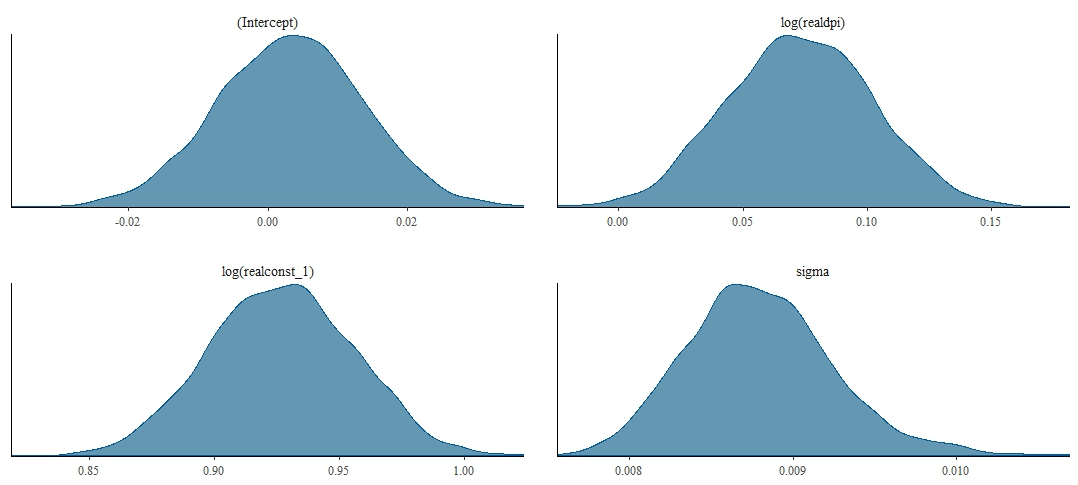
\includegraphics[width=1\linewidth]{imagenes/ej7} 


\item[c)] Obtenga la distribución posterior de $\beta_2 / (1- \beta_3)$ y un intervalo de credibilidad del $95\%$.

\begin{verbatim}
summary(hipotesis, c(0.025, 0.975))
   Min. 1st Qu.  Median    Mean 3rd Qu.    Max. 
-5.8327  0.9823  0.9946  0.9912  1.0058  3.6823 
\end{verbatim}
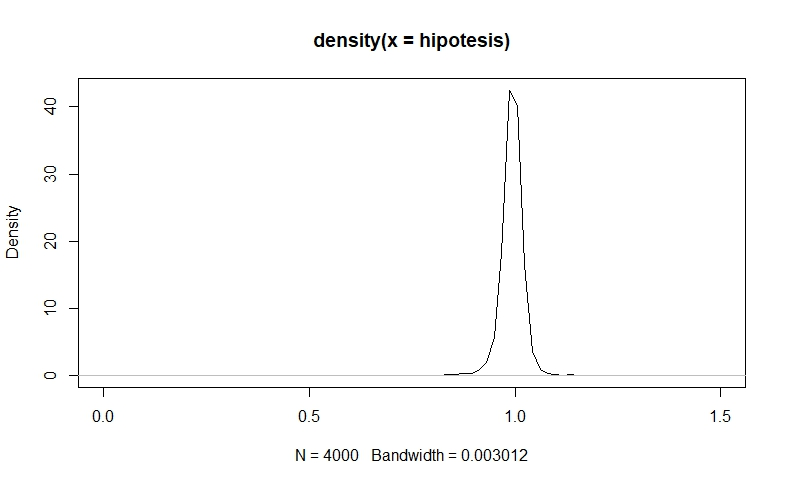
\includegraphics[width=1\linewidth]{imagenes/ej7_2} 
Dado que el intervalo contiene al 1, no hay evidencia suficiente para rechazar $H_{0}$. Por lo que se concluye que $H_{0}: \beta_{2}/(1 -\beta_{3}) = 1$, esto coincide con la conclusión del ejercicio 6.\\



\end{itemize}






%--------EJERCICIO 8------------
\paragraph{Problema 8 } ( Regresion Bayesiana).
\\
Del articulo:\\

Ellison, A. M. (2004). Bayesian inference in ecology. Ecology letters, 7(6), 509-520.\\

https://onlinelibrary.wiley.com/doi/pdf/10.1111/j.1461-0248.2004.00603.x\\
\begin{enumerate}
\item 
\begin{enumerate}
\item Realice el analsis de regresión clasico para datos de hormigas.

El modelo que se propone en el artículo es: $$log(\hat{S_{i}})=\hat{\beta_{0}}+\hat{\beta_{1}}*latitude_{i}+\hat{\beta_{2}}*elevation_{i}+\hat{\beta_{3}}habitat_{i}$$
\begin{verbatim}
> #Modelo de regresión simple
> model_reg= lm(log(Species.richness) ~ Latitude + Elevation 
+ habitat,data=datos8)
> summary(model_reg)

Call:
lm(formula = log(Species.richness) ~ Latitude + Elevation + habitat, 
    data = datos8)

Residuals:
     Min       1Q   Median       3Q      Max 
-1.10279 -0.23082  0.01417  0.25020  0.92499 

Coefficients:
                Estimate Std. Error t value Pr(>|t|)    
(Intercept)   10.3180285  2.6101963   3.953 0.000306 ***
Latitude      -0.2007838  0.0609920  -3.292 0.002085 ** 
Elevation     -0.0010856  0.0004049  -2.681 0.010610 *  
habitatForest  0.6898845  0.1269432   5.435 2.94e-06 ***
---
Signif. codes:  0 ‘***’ 0.001 ‘**’ 0.01 ‘*’ 0.05 ‘.’ 0.1 ‘ ’ 1

Residual standard error: 0.421 on 40 degrees of freedom
Multiple R-squared:  0.5625,	Adjusted R-squared:  0.5297 
F-statistic: 17.14 on 3 and 40 DF,  p-value: 2.595e-07

\end{verbatim}
\item Realice el análisis bayesiano propuesto en el paper para datos de hormigas. Use el software que considere conveniente no solo Bugs.

\begin{verbatim}
#Modelo Bayesiano con brm
model_bayes <- brm(log(Species.richness) ~ Latitude + Elevation 
                   + habitat, data = datos8)
> print(model_bayes, digits = 6)
 Family: gaussian 
  Links: mu = identity; sigma = identity 
Formula: log(Species.richness) ~ Latitude + Elevation + habitat 
   Data: datos8 (Number of observations: 44) 
  Draws: 4 chains, each with iter = 2000; warmup = 1000; thin = 1;
         total post-warmup draws = 4000

Regression Coefficients:
               Estimate Est.Error  l-95% CI  u-95% CI     Rhat
Intercept     10.333886  2.744553  4.851067 15.606958 1.002378
Latitude      -0.201223  0.064082 -0.325076 -0.073709 1.001961
Elevation     -0.001073  0.000421 -0.001913 -0.000243 1.000672
habitatForest  0.690287  0.129543  0.428947  0.942747 1.002618
              Bulk_ESS Tail_ESS
Intercept         3288     2407
Latitude          3316     2504
Elevation         4050     2824
habitatForest     3139     1939

Further Distributional Parameters:
      Estimate Est.Error l-95% CI u-95% CI     Rhat Bulk_ESS Tail_ESS
sigma 0.434155  0.049426 0.349372 0.544991 0.999932     2749     2145

Draws were sampled using sampling(NUTS). For each parameter, Bulk_ESS
and Tail_ESS are effective sample size measures, and Rhat is the potential
scale reduction factor on split chains (at convergence, Rhat = 1).

#con INLA
inlamod <- inla(log(Species.richness) ~ Latitude + Elevation 
                + habitat, data = datos8, family="gaussian")
> inlamod$summary.fixed[,1:2]
                      mean           sd
(Intercept)   10.318001469 2.6118938902
Latitude      -0.200783076 0.0610316371
Elevation     -0.001085631 0.0004051898
habitatForest  0.689873401 0.1270249233

#Con Stan
model_bayes<- stan_glm(log(Species.richness) ~ Latitude + Elevation 
                       + habitat, data = datos8, seed=111)
> print(model_bayes, digits = 3)
 Family: gaussian 
  Links: mu = identity; sigma = identity 
Formula: log(Species.richness) ~ Latitude + Elevation + habitat 
   Data: datos8 (Number of observations: 44) 
  Draws: 4 chains, each with iter = 2000; warmup = 1000; thin = 1;
         total post-warmup draws = 4000

Regression Coefficients:
              Estimate Est.Error l-95% CI u-95% CI  Rhat Bulk_ESS
Intercept       10.334     2.745    4.851   15.607 1.002     3288
Latitude        -0.201     0.064   -0.325   -0.074 1.002     3316
Elevation       -0.001     0.000   -0.002   -0.000 1.001     4050
habitatForest    0.690     0.130    0.429    0.943 1.003     3139
              Tail_ESS
Intercept         2407
Latitude          2504
Elevation         2824
habitatForest     1939

Further Distributional Parameters:
      Estimate Est.Error l-95% CI u-95% CI  Rhat Bulk_ESS Tail_ESS
sigma    0.434     0.049    0.349    0.545 1.000     2749     2145

Draws were sampled using sampling(NUTS). For each parameter, Bulk_ESS
and Tail_ESS are effective sample size measures, and Rhat is the potential
scale reduction factor on split chains (at convergence, Rhat = 1).
\end{verbatim}

En ambos modelos, tanto de regresión simple como de regresión bayesiana se obtienen valores de los estimadores muy simulares.
\end{enumerate}
\end{enumerate}

\end{document}